\part{Expectativas}
\chapter[Conclusões]{Conclusões}
De acordo com as informações pesquisadas e apresentadas neste relatório, verificou-se que o projeto, até o momento, é viável e, ainda, percebeu-se a importância do novo prédio para comunidade da Faculdade do Gama, pois este é capaz de sanar problemas existentes na FGA.

\section{Próximos Pontos de Controle}

Para o próximo ponto de controle serão aprofundados os estudos dos riscos e demandas identificados no projeto. Ainda serão realizadas as representações dos sistemas usados no prédio e do prédio em si além da simulação de um dos sistemas, os dispositivos de acesso e presença.

Além disso, serão feitas ainda as simulações de consumo e produção de energia, simulação dos eletrônicos de instrumentação e controle. Nesse ponto de controle o foco será mostrar a viabilidade econômica do projeto através das estimativas de payback, dos custos de cada segmento trabalhado.

\section{Cronograma do Projeto}
\begin{figure}[!h]
 \centering	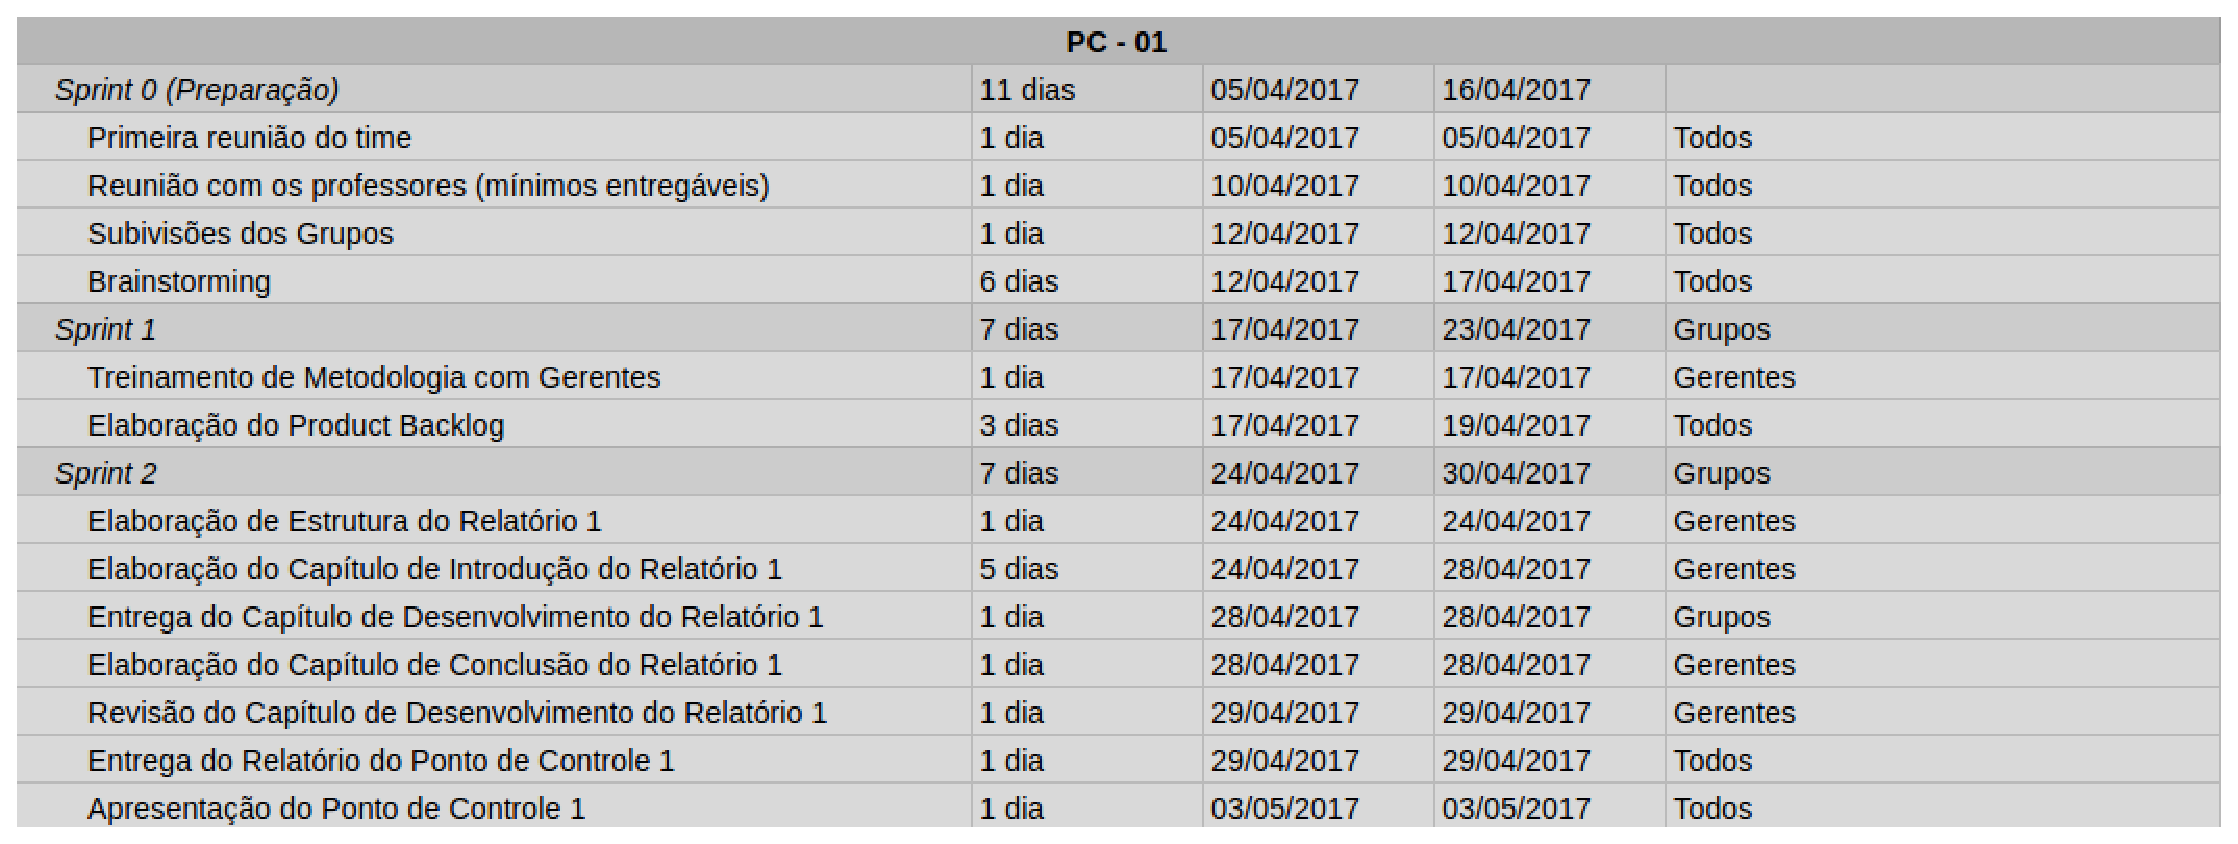
\includegraphics[keepaspectratio=true,scale=0.45]{figuras/c1.eps}
 \caption{Cronograma do Projeto - Parte 1}
 \label{fig022}
\end{figure}
\pagebreak
\begin{figure}[!h]
 \centering	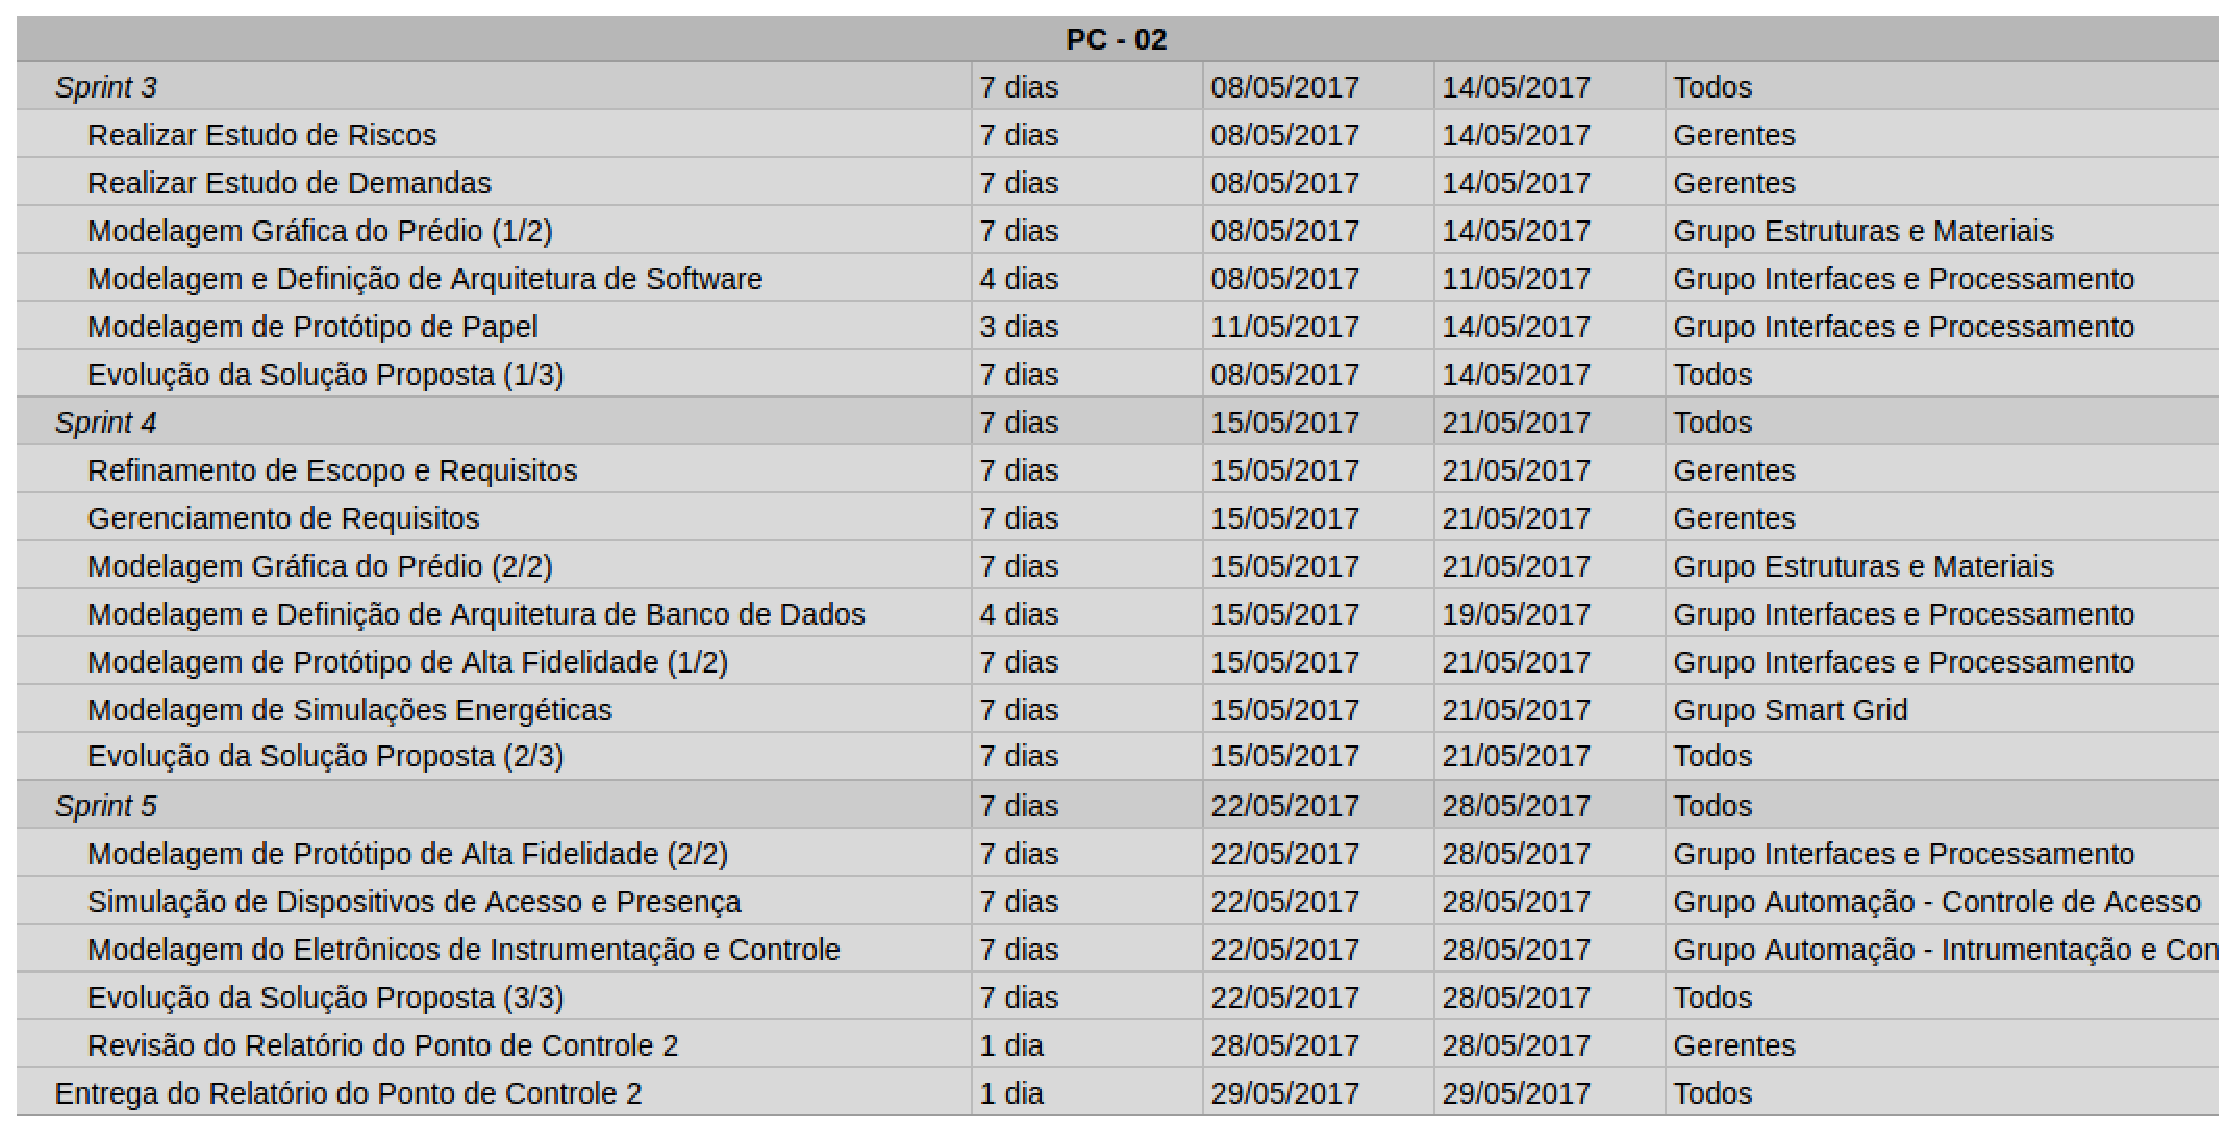
\includegraphics[keepaspectratio=true,scale=0.45]{figuras/c2.eps}
 \caption{Cronograma do Projeto - Parte 2}
 \label{fig022}
\end{figure}

\begin{figure}[!h]
 \centering	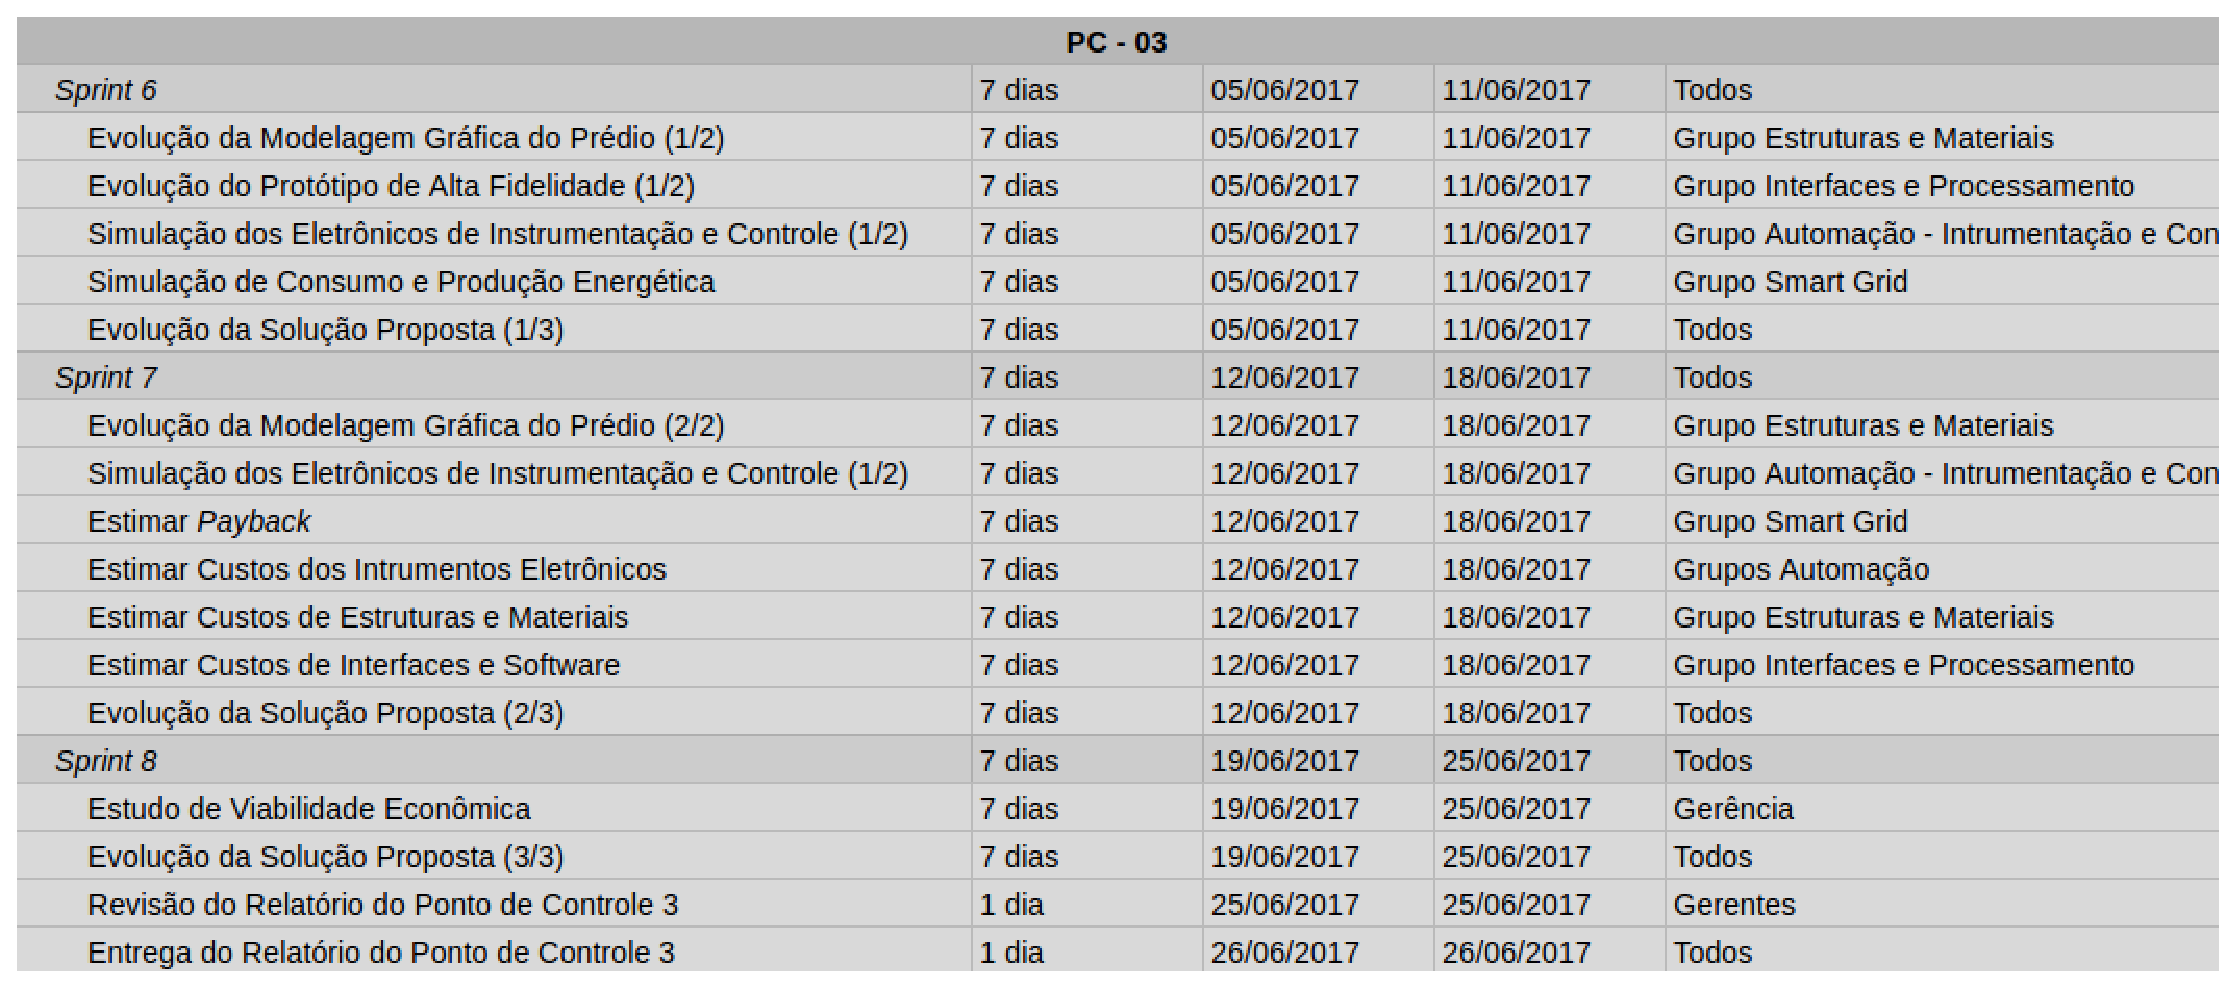
\includegraphics[keepaspectratio=true,scale=0.45]{figuras/c3.eps}
 \caption{Cronograma do Projeto - Parte 3}
 \label{fig022}
\end{figure}
